\section{SN: EEG}
\label{sec:EEG}
\ghnote{Solveig and Torbjørn will write this chapter.}

\subsection{\red{From transmembrane currents to current dipoles}}
In calculation of LFPs, we relied on current sources and sinks, typically in an infinite homogeneous medium. But calculations of EEG signals require head models, and to the best of our knowledge, all existing head model take current dipoles as input instead of current sources and sinks. It is however possible to go from neuronal transmembrane currents to neuronal current dipoles \citep{Naess2020}.

\begin{figure}[!ht]
\begin{center}
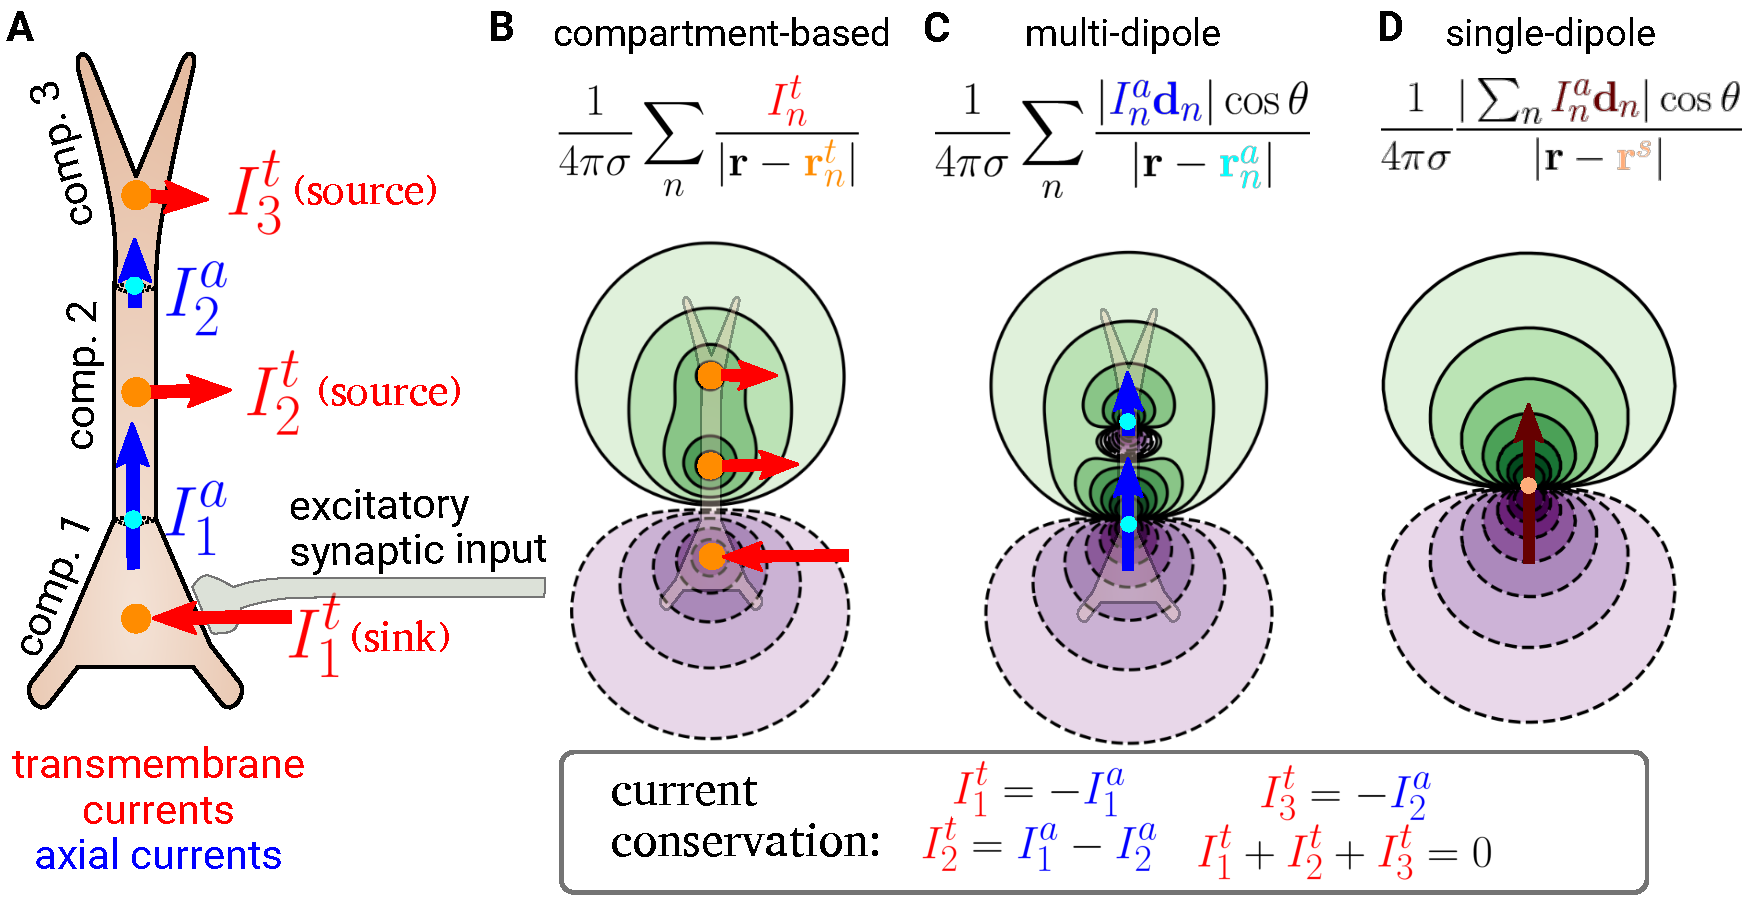
\includegraphics[width=0.8\textwidth]{Figures/EEG/illustration_imem_iaxial.pdf}
\end{center}
\caption{\textbf{Different approaches to calculating extracellular potentials} 
}
\label{VC:fig:pointsource}
\end{figure}

\subsection{\red{SN: 4-sphere model}} 
Kjernereferanse: \citep{Naess2017} and \citep{Naess2020}.

\subsection{\red{Complex head models}} 
It is possible to use pre-solved complex head models, like the New York Head model.

\subsection{\red{Differences between EEG and LFP signals}}
EEG is simpler because it is far away (Fig.~\ref{EEG:fig:simple_EEG}).
\begin{figure}[!ht]
\begin{center}
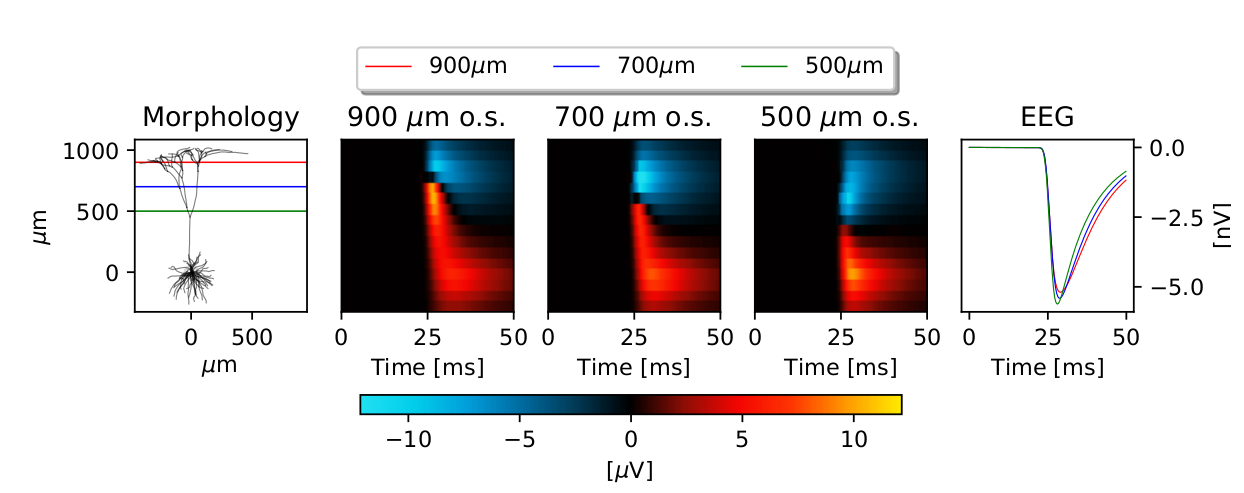
\includegraphics[width=0.8\textwidth]{Figures/EEG/EEG_is_simple.png}
\end{center}
\caption{\textbf{[Placeholder, from JFK] EEG is simpler than LFP} 
LFP is much more dependend on details of synaptic input
}
\label{EEG:fig:simple_EEG}
\end{figure}



\subsection{\red{SN: Insights from EEG studies} }
